\documentclass[10pt, hyperref={pdfpagelabels=false}]{beamer}

% Configuración
\usepackage[utf8]{inputenc}
\usepackage[spanish]{babel}
\usepackage{lmodern} % Arregla un warning
\usepackage{multicol}

% Tema beamer
\usetheme{Warsaw}

% Detalles
\title[Asesorías Académicas]{Aplicación web para la gestión de la Asesoría
                             Académica en la Universidad de Córdoba}
\author{Bartolomé Sánchez Salado}
\institute{
    \begin{tabular}{lp{3cm}r}
      \textbf{Director} && \\
      Nicolás Luis Fernández García && \scriptsize{Córdoba, enero 2011} \\
    \end{tabular}}
\date{}

\begin{document}

  %--- PORTADA ---%
  \begin{frame}[plain]
    \begin{tabular}{ccc}
      \\
      
\includegraphics[height=0.18\textheight]{uco} &
      \begin{tabular}{c}
        {\bf UNIVERSIDAD DE CÓRDOBA} \\
        {\bf Escuela Politécnica Superior} \\\\
        Ingeniería Técnica en Informática de Gestión \\
        Proyecto de fin de carrera \\\\
        \end{tabular} &
      
\includegraphics[height=0.18\textheight]{eps} \\
    \end{tabular}
    \titlepage
  \end{frame}

  \AtBeginSection[]
  {
    \begin{frame}<beamer>
      \frametitle{Sumario}
      \tableofcontents[currentsection,hideallsubsections]
    \end{frame}
  }

  \AtBeginSubsection[]
  {
    \begin{frame}<beamer>
      \frametitle{Contenido de la sección}
      \begin{multicols}{2}
        \tableofcontents[currentsubsection,subsectionstyle=show/shaded/hide]
      \end{multicols}
    \end{frame}
   }

   \begin{frame}{Contenido}
    \tableofcontents[hideallsubsections]
   \end{frame}

  \section{Presentación}
    \subsection{Introducción}
      \begin{frame}{Introducción}
        \begin{block}{Asesoría clásica}
          \begin{itemize}
          \item Se limitaba a tutorías.
          \item Siempre dentro del ámbito de una asignatura.
          \end{itemize}
        \end{block}
        \onslide<2->
        \begin{block}{Asesoría Académica}
          \begin{itemize}
          \item Tiene una aplicación más amplia y genérica.
          \item Aparece la figura del Asesor Académico.
          \end{itemize}
        \end{block}
      \end{frame}

      \begin{frame}{Introducción}
        \begin{block}{Asesor Académico}
          \begin{itemize}
           \item Orienta al estudiante durante su estancia en la Universidad.
           \item Realiza un seguimiento del alumno:
           \begin{itemize}
            \item Permanente.
            \item Eficaz.
            \item Orientado a la optimización del esfuerzo de estudio.
           \end{itemize}
          \end{itemize}
        \end{block}
      \end{frame}

      \begin{frame}{Introducción}
        \begin{block}{Asesoría Académica en la UCO}
          \begin{itemize}
           \item En marzo de 2007, a través del Plan Propio de Calidad de la
                 Enseñanza, se contempla la creación de la figura del Asesor
                 Académico.
          \end{itemize}
        \end{block}
        \onslide<2->
        \begin{block}{Asesoría Académica en la UCO}
          \begin{itemize}
           \item Se establece un reglamento regulador:
           \begin{itemize}
            \item Guías.
            \item Fichas.
           \end{itemize}
          \end{itemize}
        \end{block}
      \end{frame}


    \subsection{Definición del problema}
      \begin{frame}{Definición del problema}
        \begin{block}{Problema}
          \begin{itemize}
           \item Reciente implantación del Asesor Académico.
           \begin{itemize}
            \item Organización de la información poco eficiente.
           \end{itemize}
          \end{itemize}
         \end{block}
           \onslide<2->
         \begin{block}{Dificultades}
          \begin{itemize}
           \item Guías y fichas en papel:
           \begin{itemize}
            \item Gran cantidad de información.
            \item Acceso.
            \item Actualización/modificación.
           \end{itemize}
          \end{itemize}
        \end{block}
      \end{frame}

      \begin{frame}{Definición del problema}
        \begin{block}{Necesidad de un sistema de gestión}
          \begin{itemize}
           \item Fácil acceso a la información.
           \item Almacenamiento.
           \item Fácil manipulación de los datos.
           \item Interactividad.
          \end{itemize}
        \end{block}
      \end{frame}


    \subsection{Objetivos}
      \begin{frame}{Objetivos}
        \begin{block}{Objetivo general}
        Crear un sistema que gestione toda la información relativa a la Asesoría
        Académica.
        \end{block}
      \end{frame}

      \begin{frame}{Objetivos}
        \begin{block}{Objetivos específicos}
          \begin{itemize}
           \item Gestión de la información personal de los alumnos.
           \item Herramientas para facilitar el seguimiento a los alumnos.
           \item Realización de entrevistas.
           \begin{itemize}
            \item Individuales.
            \item Grupales.
           \end{itemize}
           \item Consultas.
           \item Generación de informes.
           \item Copias de seguridad.
          \end{itemize}
        \end{block}
      \end{frame}


    \subsection{Antecedentes}
      \begin{frame}{Antecedentes}
        \begin{block}{Aplicaciones informáticas}
          \begin{itemize}
           \item \textbf{Portal para la Asesoría Académica}.
           \begin{itemize}
            \item Proyecto de fin de carrera.
            \item I.T. Informática de Sistemas, 2010.
            \item Autor:
            \begin{itemize}
              \item Carmona Varo, F.
            \end{itemize}
            \item Director:
            \begin{itemize}
              \item Cerruela García, G.
            \end{itemize}
           \end{itemize}
          \end{itemize}
        \end{block}
      \end{frame}

      \begin{frame}{Portal para la Asesoría Académica}
        \begin{block}{Inconvenientes}
          \begin{itemize}
           \item Información desorganizada.
           \item No se tienen en cuenta:
           \begin{itemize}
            \item Centros.
            \item Titulaciones.
            \item Asignaturas.
           \end{itemize}
          \end{itemize}
        \end{block}
        \onslide<2->
        \begin{block}{Inconvenientes}
          \begin{itemize}
           \item No hace distinción por curso académico:
           \begin{itemize}
            \item Complica el estudio de la evolución temporal de
                  acontecimientos.
           \end{itemize}
           \item Sin posibilidad de preguntas de asesor propias.
           \begin{itemize}
            \item Únicamente preguntas del sistema.
           \end{itemize}
          \end{itemize}
        \end{block}
      \end{frame}


    \subsection{Restricciones}
      \begin{frame}{Restricciones}
        \begin{block}{Factores iniciales}
          \begin{itemize}
            \item Tener en cuenta la información que proporciona el
                  Vicerrectorado de Planificación y Calidad de la UCO.
            \item Multiplataforma.
            \item Acceso al sistema personalizado: roles.
            \item Interfaz gráfica fácil e intuitiva.
            \item Uso de un sistema de control de versiones para el desarrollo.
            \begin{itemize}
            \item \textit{Subversion}.
            \end{itemize}
          \end{itemize}
        \end{block}
      \end{frame}

      \begin{frame}{Restricciones}
        \begin{block}{Factores estratégicos}
          \begin{itemize}
           \item Debian GNU/Linux.
           \item XHTML.
           \item Python - Django.
           \item PostgreSQL.
          \end{itemize}
        \end{block}
      \end{frame}


    \subsection{Recursos}
      \begin{frame}{Recursos}
        \begin{block}{Recursos humanos}
          \begin{itemize}
           \item \textbf{Autor:} Bartolomé Sánchez Salado.
           \item \textbf{Director:} Nicolás Luis Fernández García.
          \end{itemize}
        \end{block}
      \end{frame}

      \begin{frame}{Recursos}
        \begin{block}{Recursos hardware}
          \begin{itemize}
            \item Ordenador personal:
            \begin{itemize}
              \item Intel Pentium 4 CPU 2.40 Ghz.
              \item 768 MB de memoria RAM.
              \item 30 GB de disco duro.
            \end{itemize}
            \onslide<2->
            \item Servidor (gestor de versiones):
            \begin{itemize}
              \item Intel Celeron CPU 800 Mhz.
              \item 256 MB de memoria RAM.
              \item 40 GB de disco duro.
            \end{itemize}
          \end{itemize}
        \end{block}
      \end{frame}

      \begin{frame}{Recursos}
        \begin{block}{Recursos software (I)}
          \begin{itemize}
           \item Sistemas operativos.
           \begin{itemize}
            \item Debian GNU/Linux 6.0 (Squeeze).
            \item Debian GNU/Linux 5.0 (Lenny).
           \end{itemize}
           \item Sistema de control de versiones.
           \begin{itemize}
            \item \textit{Subversion}.
           \end{itemize}
           \item Desarrollo software.
           \begin{itemize}
            \item Kate.
            \item Python.
            \item Django.
           \end{itemize}
          \end{itemize}
        \end{block}
      \end{frame}

      \begin{frame}{Recursos}
        \begin{block}{Recursos software (II)}
          \begin{itemize}
           \item Gestión base de datos.
           \begin{itemize}
            \item PostgreSQL.
           \end{itemize}
           \item Servidor web.
           \begin{itemize}
            \item Apache (módulo \textit{mod\_wsgi})
           \end{itemize}
           \item Edición y visualización.
           \begin{itemize}
            \item Latex.
            \item Kile.
           \end{itemize}
          \end{itemize}
        \end{block}
      \end{frame}


  \section{Análisis}
    \subsection{Especificación de requisitos}
      \begin{frame}{Especificación de requisitos}
        \begin{block}{Gestión de la Asesoría Académica.}
          \begin{itemize}
           \item Módulo de administrador principal.
           \item Módulo de administrador de centro.
           \item Módulo de asesores.
           \item Módulo de alumnos.
          \end{itemize}
        \end{block}
      \end{frame}

      \begin{frame}{Especificación de requisitos}
        \begin{block}{Módulo de administrador principal.}
          \begin{itemize}
           \item Gestión del sistema.
           \item Gestión de plantillas de entrevista institucionales.
           \item Gestión de copias de seguridad.
           \item Explotación del sistema.
           \item Ayuda.
          \end{itemize}
        \end{block}
      \end{frame}

      \begin{frame}{Especificación de requisitos}
        \begin{block}{Módulo de administrador de centro.}
          \begin{itemize}
           \item Gestión de centro.
           \item Explotación del sistema.
           \item Ayuda.
          \end{itemize}
        \end{block}
      \end{frame}

      \begin{frame}{Especificación de requisitos}
        \begin{block}{Módulo de asesores.}
          \begin{itemize}
           \item Gestión de alumnos.
           \item Gestión de plantillas de entrevista de asesor.
           \item Gestión de entrevistas.
           \item Explotación del sistema.
           \item Ayuda.
          \end{itemize}
        \end{block}
      \end{frame}

      \begin{frame}{Especificación de requisitos}
        \begin{block}{Módulo de alumnos.}
          \begin{itemize}
           \item Explotación del sistema.
           \item Ayuda.
          \end{itemize}
        \end{block}
      \end{frame}

      \begin{frame}{Especificación de requisitos}
        \begin{block}{Supuestos semánticos.}
          \begin{multicols}{2}
          \begin{itemize}
           \item Centro.
           \item Titulación.
           \item Asignatura.
           \item Alumno.
           \item Asesor.
           \item Administrador de centro.
           \item Departamento.
           \item Reunión.
           \item Plantilla Entrevista Oficial.
           \item Plantilla Entrevista Asesor.
           \item Pregunta Oficial.
           \item Pregunta Asesor.
          \end{itemize}
          \end{multicols}
        \end{block}
      \end{frame}

      \begin{frame}{Especificación de requisitos}
        \begin{block}{Ejemplos de supuestos semánticos}
          \begin{itemize}
            \item \textit{Una asignatura tiene asignada una carga docente
                  traducida en un número de créditos, teóricos y prácticos.}
            \item \textit{Una reunión puede ser individual, donde solo
                  participará un usuario alumno, o grupal, donde pueden
                  participar varios.}
          \end{itemize}
        \end{block}
      \end{frame}


    \subsection{Modelización de la información}
      \begin{frame}{Modelo Entidad-Relación}
        \begin{center}
          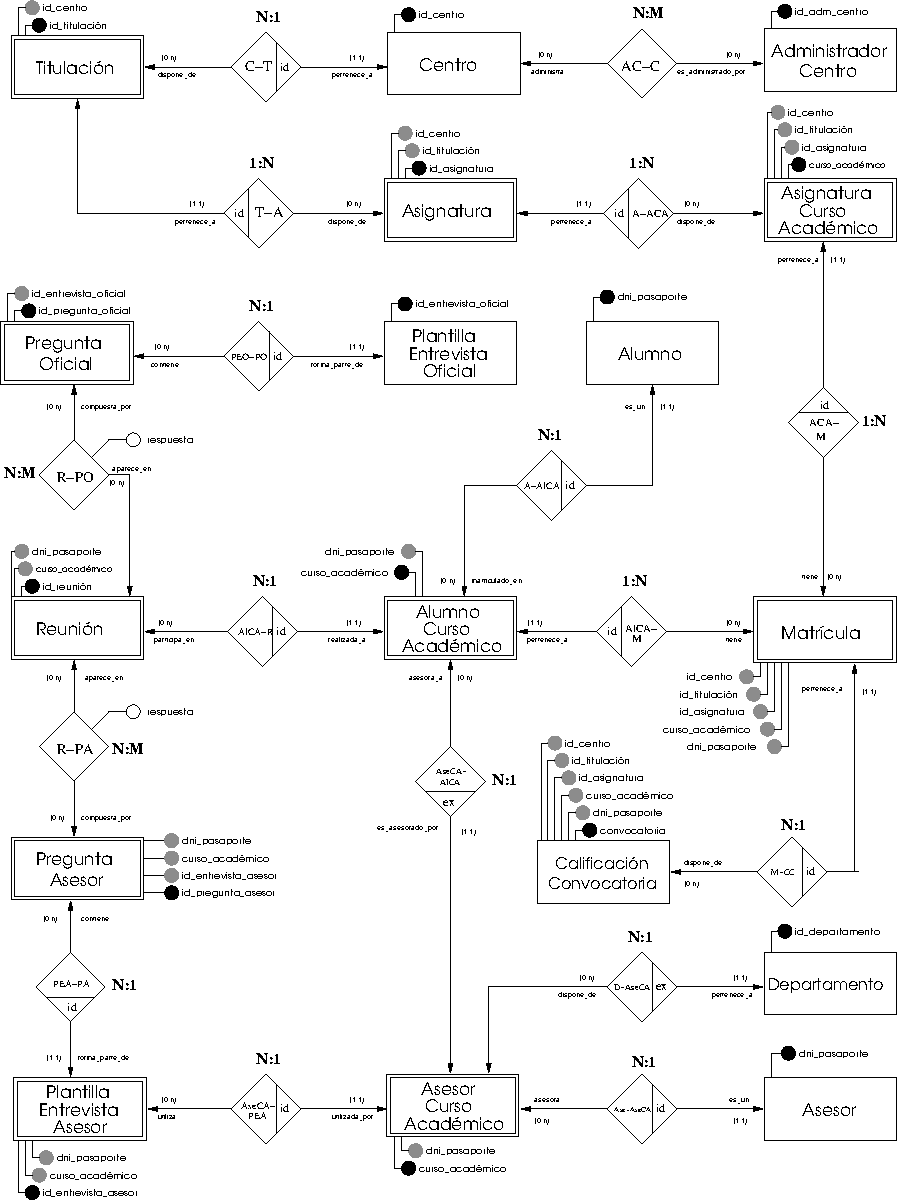
\includegraphics[height=6.5cm]{Diagramas/diagramaER}
        \end{center}
      \end{frame}

    \subsection{Descripción funcional}
      \begin{frame}{Descripción funcional}

      \end{frame}


  \section{Diseño}
    \subsection{Diseño de datos}
      \begin{frame}{Diseño de datos}
        \begin{block}{Proceso}
          \begin{itemize}
            \item Obtención de las tablas.
            \item Normalización.
          \end{itemize}
        \end{block}
        
\begin{center}
\begin{table}[H]
\begin{center}
\scriptsize
\begin{tabular}{p{4cm}p{4cm}}

\hline
\textbf{Tablas} & \\
\hline
\hline

\textbf{Centros} &
\textbf{Alumnos} \\

\textbf{AdministradoresCentro} &
\textbf{AlumnosCursoAcadémico} \\

\textbf{Titulaciones} &
\textbf{Matrículas} \\

\textbf{Asignaturas} &
\textbf{CalificacionesConvocatoria} \\

\textbf{AsignaturasCursoAcadémico} &
\textbf{PlantillasEntrevistaOficial} \\

\textbf{Departamentos} &
\textbf{PreguntasOficiales} \\

\textbf{Asesores} &
\textbf{Reuniones} \\

\textbf{AsesoresCursoAcadémico} &
\textbf{Centro\_AdministradoresCentro} \\

\textbf{PlantillasEntrevistaAsesor} &
\textbf{Reunión\_PreguntasAsesores} \\

\textbf{PreguntasAsesores} &
\textbf{Reunión\_PreguntasOficiales} \\

\\
\hline
& \textbf{\tiny20 tablas en total}\\

\end{tabular}
\end{center}
\end{table}
\end{center}
      \end{frame}

    \subsection{Diseño arquitectónico}
      \begin{frame}{Diseño arquitectónico}
        \begin{center}
          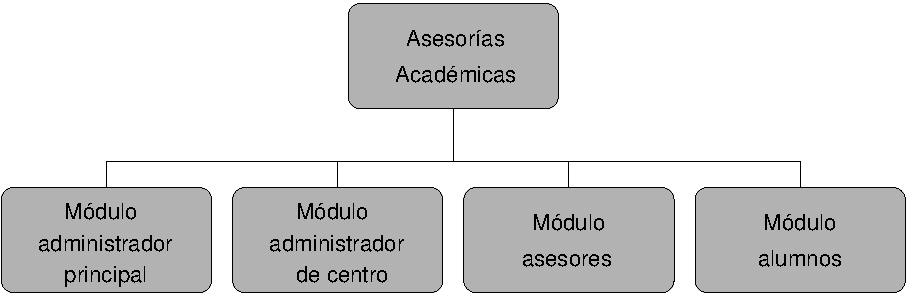
\includegraphics[width=9cm]{Diagramas/disenyoArquitectonico}
        \end{center}
      \end{frame}

      \begin{frame}{Módulo Administrador principal}
        \begin{center}
          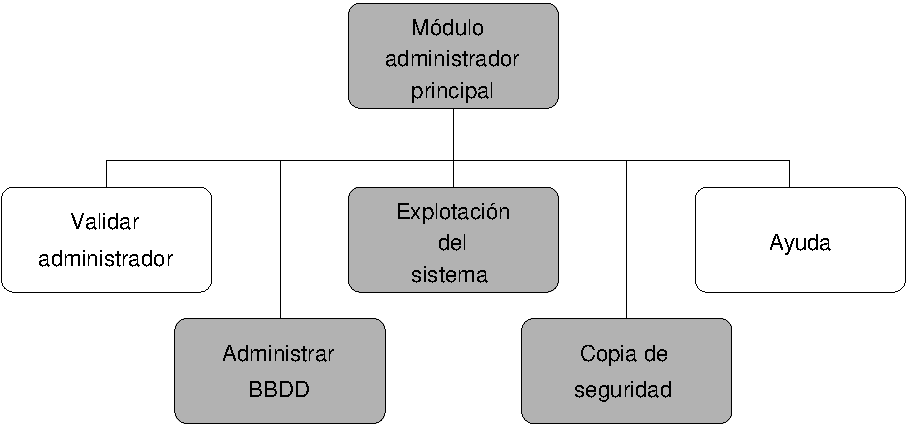
\includegraphics[width=9cm]{Diagramas/moduloAdminPrincipal}
        \end{center}
      \end{frame}

      \begin{frame}{Módulo Administrador de centro}
        \begin{center}
          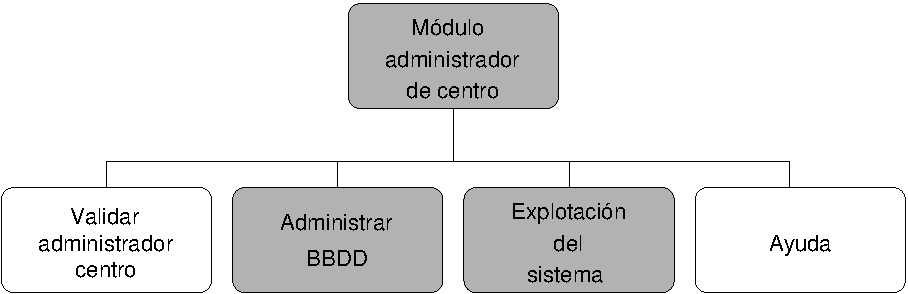
\includegraphics[width=9cm]{Diagramas/moduloAdminCentro}
        \end{center}
      \end{frame}

      \begin{frame}{Módulo Asesores}
        \begin{center}
          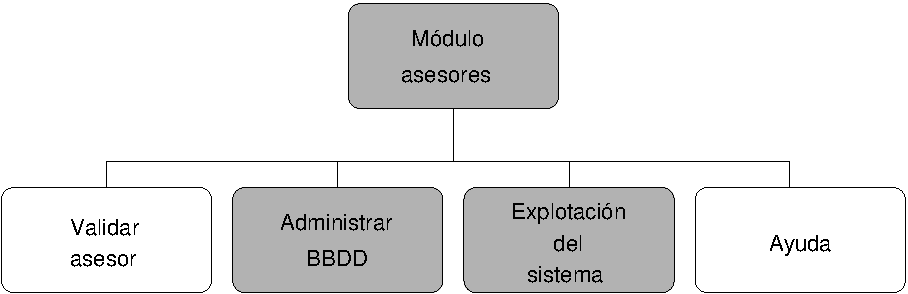
\includegraphics[width=9cm]{Diagramas/moduloAsesores}
        \end{center}
      \end{frame}

      \begin{frame}{Módulo Alumnos}
        \begin{center}
          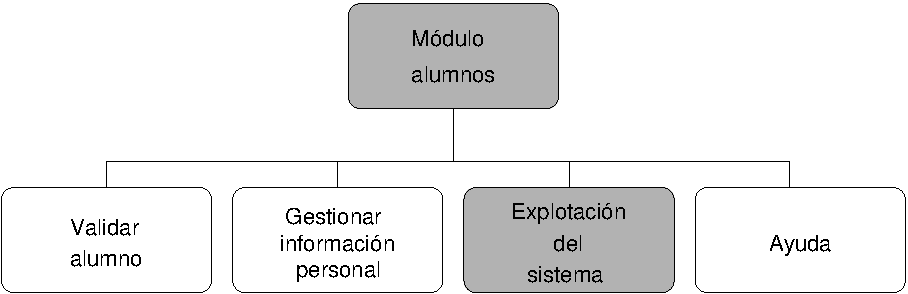
\includegraphics[width=9cm]{Diagramas/moduloAlumnos}
        \end{center}
      \end{frame}

    \subsection{Diseño de la interfaz}
      \begin{frame}{Diseño de la interfaz}
        \begin{center}
          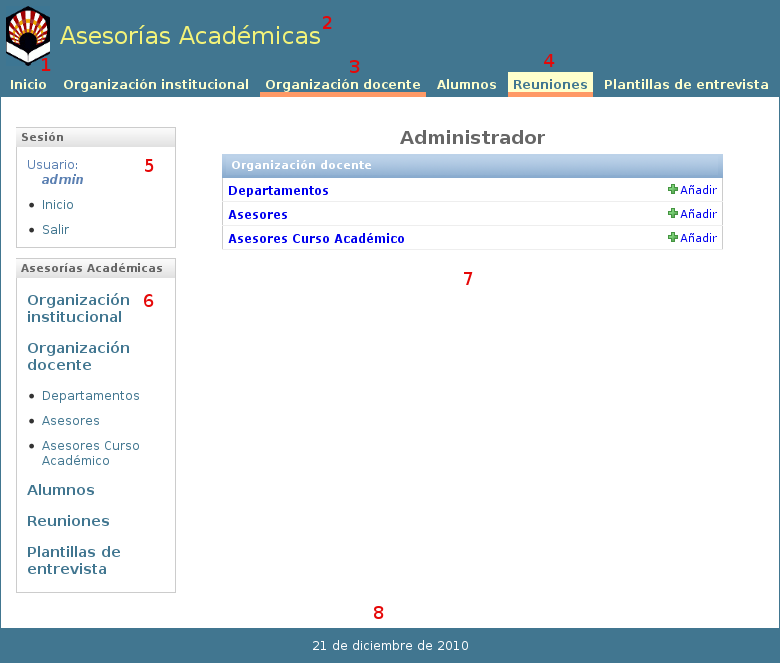
\includegraphics[height=6.5cm]{Diagramas/gestion_informacion.png}
        \end{center}
      \end{frame}


  \section{Pruebas del software}
    \begin{frame}{Pruebas del software}

    \end{frame}


  \section{Demostración del sistema}
    \begin{frame}{Demostración del sistema}

    \end{frame}


  \section{Conclusiones}
    \subsection{Conclusiones}
      \begin{frame}{Conclusiones}

      \end{frame}

    \subsection{Futuras mejoras}
      \begin{frame}{Futuras mejoras}

      \end{frame}

\end{document}